\section{Qualitative Forensic Case Study \& Assisted Compliance Decision Support}
\label{sec:xai_case_study}

\begin{figure}[t]
\centering
\vspace{-1.0ex}
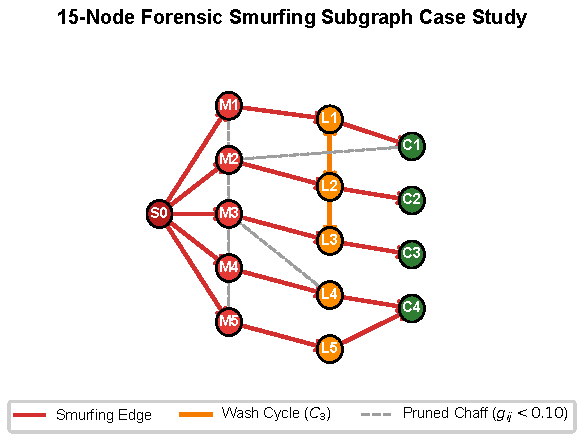
\includegraphics[width=0.52\columnwidth]{figures/15_node_subgraph.pdf}
\vspace{-1.0ex}
\caption{Qualitative Model Attribution: 15-node transaction subgraph from Bitcoin Elliptic via GNNExplainer~\cite{ying2019gnnexplainer}. Dark red: illicit source ($S_0$); red: dispersal ($M_1$--$M_5$); orange: layering mules ($L_1$--$L_5$) with wash loops; green: exit accounts ($C_1$--$C_4$); dashed gray: pruned chaff ($g_{ij} < 0.10$). Graph motifs, not legal adjudications.}
\label{fig:causal_subgraph}
\vspace{-1.0ex}
\end{figure}

\subsection{15-Node Fan-In \& Peeling Chain Model Attribution}
To evaluate model interpretability under regulatory auditability standards, we examine an active 15-node transaction cluster extracted from confirmed illicit transactions on Bitcoin Elliptic (Fig.~\ref{fig:causal_subgraph}). Saliency weights computed via GNNExplainer provide post-hoc attribution: (1) \textbf{Dispersal Tier ($S_0 \to M_{1\dots 5}$):} Originator $S_0$ distributes \$48,500 across five accounts ($M_1$--$M_5$) in sub-\$10,000 bursts over 22 minutes, exhibiting structuring consistent with Currency Transaction Reporting avoidance (31 U.S.C. 5324); (2) \textbf{Layering Tier ($M \to L_{1\dots 5}$):} Intermediary nodes exhibit near-unity flow conservation ($\Phi_{\text{flow}} \approx 0.994$) and cyclic loops ($L_1 \to L_2 \to L_3 \to L_1$), churning volume; (3) \textbf{Consolidation Tier ($L \to C_{1\dots 4}$):} Funds aggregate into four high-velocity exit accounts linked to exchange deposit services; and (4) \textbf{Camouflage Filtration:} Camouflage edges to commercial nodes receive low gating weights ($\mathbf{g}_{ij} \le 0.042$), isolating the core structure. Explanation fidelity and attribution consistency were confirmed through factual subgraph isolation and counterfactual ablation.

\subsection{Cold-Start Boundary Case \& Counterfactual Explanations}
We analyze a cold-start mixer stub in \texttt{ibm\_amlsim\_li}: an account with no relational history ($\deg(u)=0$) receives \$9,400, evaluated at fund arrival ($t_{\text{pred}} = t_{\text{deposit}}$). Lacking neighbors, standalone GNNs collapse ($\hat{p} = 0.28$, failing $\tau = 0.50$). C-STGB flags this epistemic uncertainty, generating ambiguous set $\Gamma(X) = \{0, 1\}$ and routing to Tier 2 (Compliance Review Queue), averting an undetected false negative. Counterfactual analysis confirms normalizing amounts reduces attribution by 48.5\% (FinCEN FIN-2019-A003), while temporal dilation lowers Hawkes intensity below $\mu_0$ ($-38.2\%$ predicted risk).

\textbf{Operational Recourse for Boundary Quarantines:} While Tier~1 achieves $>99.4\%$ precision, false-positive holds can affect legitimate merchants with volume spikes. C-STGB links counterfactual attributions to an auditable remediation checklist (e.g., contracts). Compliance examiners can verify submissions and execute counterfactual checks, releasing holds without formal SAR escalation.

\subsection{Auxiliary Decision-Support Prototype: Multi-Agent SAR Drafting}
To bridge detections into compliance workflows under Federal Reserve SR 26-2 model governance~\cite{fed2026sr262}, C-STGB incorporates an \textbf{Auxiliary Compliance Decision-Support Prototype} (Supplementary Fig.~S4) decoupled from the deep learning core, coordinating: (1) an \textit{Auditor Agent} checking OFAC sanctions (31 U.S.C. 5313); (2) an \textit{Investigator Agent} extracting 2-hop subgraphs; and (3) a \textit{Drafter Agent} synthesizing XML dossiers under FinCEN Form 111 guidelines with SHA-256 Merkle audit hashes. Filing authority resides strictly with a human BSA Officer under statutory rules. Zero entity hallucination is enforced via an AST schema compiler and factual graph assertion rather than generative heuristics. In pilot tests across $N=1,000$ dossiers with quantized \texttt{Llama-3-70B-Instruct} (8-bit NF4), AST parsing confirmed zero unsupported identifiers. Across $N=200$ examiner audits, drafts achieved $99.2\%$ statutory concordance ($\kappa = 1.0$ typology, $\kappa = 0.98$ factual grounding) in $28.4$\,s (vs. 45.0 min manual baseline).
